\addcontentsline{toc}{chapter}{\textsc{Anexo}}
\chapter*{Anexo}

Como Anexo se añade un ejemplo práctico de un contador de 4 bits como primera toma de contacto. Se pretende conocer los elementos 
de la tarjeta \textbf{Zybo} además de conocer las diferentes fases de flujo de diseño con Vivado.

Para abordar la fase de diseño, se ha comenzado creando un proyecto en Vivado con la siguiente descripción funcional \textit{VHDL}. Para la verificación de su 
funcionalidad se hizo una simulación de comportamiento (Ver Figura \ref{contador}).

\vspace{1cm}

\begin{lstlisting}
    library ieee;
    use ieee.std_logic_1164.all;
    use ieee.std_logic_arith.all;
    use ieee.std_logic_unsigned.all;

    entity contador_4bits is
        Port(	Reloj		: IN	std_logic;
                Reset		: IN 	std_logic;
                Salida		: OUT	std_logic_vector(3 downto 0));
    end contador_4bits;

    architecture funcional of contador_4bits IS
    signal Contador : std_logic_vector(3 downto 0):="0000"; --valores 0 a 255;
    begin
        process (Reloj, Reset)
        begin
        if Reset='1' then Contador <= "0000";
            elsif reloj'event AND reloj = '1' then Contador <= Contador + 1;			
            end if;
        end process;
        Salida <= Contador;
    end funcional;
\end{lstlisting}

Antes de la simulación, se mira la netlist resultante de la síntesis RT donde aparecen componentes genéricos 
independientes de la tecnología (Figura \ref{netlist2}).

Para poder comprobar la correcta funcionalidad del contador realizaremos una simulación de comportamiento. Para ello, 
se necesita un testbench o bien añadir las señales manualmente durante la simulación. En el siguiente testbench se 
instancia el componente que queremos simular, el contador, y añadimos un estímulopara la señal del reloj y otra para 
la del reset.

\begin{figure}[H]
    \centering
    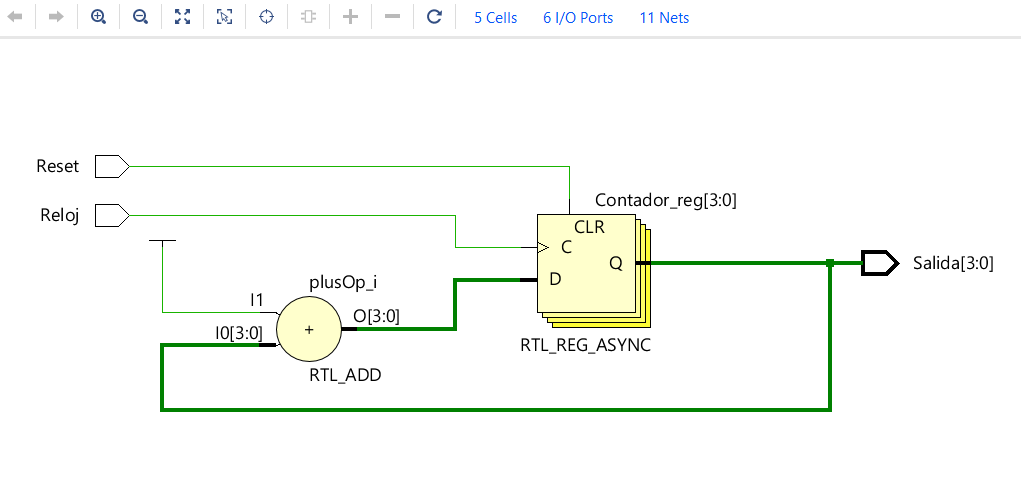
\includegraphics[width = 1\textwidth]{imagenes/netlist2.png}
    \caption{\textit{Netlist RT}}\label{netlist2}
\end{figure}

\begin{lstlisting}
    library IEEE;
use IEEE.STD_LOGIC_1164.ALL;

entity contador_4bits_tb is
end contador_4bits_tb;

architecture Behavioral of contador_4bits_tb is
    COMPONENT contador_4bits 
    PORT(
        Reloj : in std_logic;
        Reset : in std_logic;
        Salida : out std_logic_vector(3 downto 0)
    );
    END COMPONENT;
    
    SIGNAL reloj_s : std_logic := '0';
    SIGNAL reset_s : std_logic;
    SIGNAL salida_s : std_logic_vector(3 downto 0);
       
begin
    DUT : contador_4bits 
    PORT MAP(
      Reloj => reloj_s,
      Reset => reset_s,
      Salida => salida_s  
    );
    
    reloj_s <= NOT reloj_s AFTER 10ns;      -- estimulo del reloj
    
    estimulos: PROCESS
    BEGIN
        reset_s <= '1';
        WAIT FOR 10ns;
        reset_s <= '0';
        WAIT;
        
    END PROCESS;
    
end Behavioral;
\end{lstlisting}

\begin{figure}[H]
    \centering
    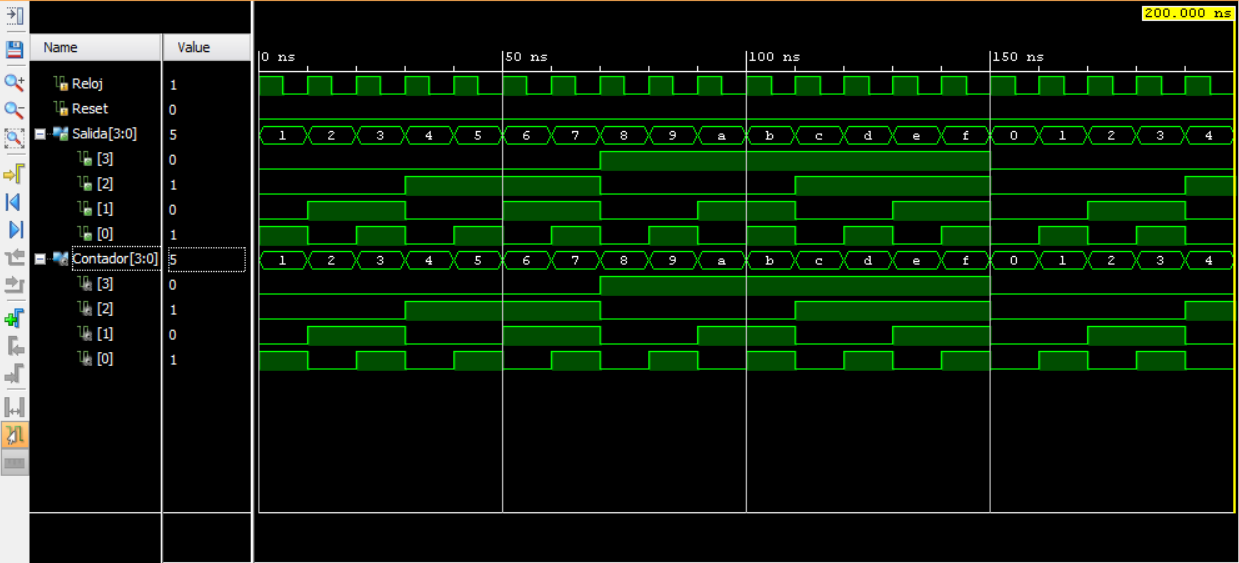
\includegraphics[width = 1\textwidth]{imagenes/contador4bits.png}
    \caption{\textit{Simulación Funcional Contador 4 Bits}}\label{contador}
\end{figure}

Si las salidas simuladas son correctas, podemos pasar a la fase de síntesis (\textit{Synthesis}). Para ello, ejecutamos la síntesis, 
y si la ejecución no ha tenido errores, entonces podremos visualizar la netlist resultante con celdas propias de la biblioteca de la 
FPGA asignada al proyecto (la de la tarjeta Zybo) (Ver Figura \ref{netlist}).

\begin{figure}[H]
    \centering
    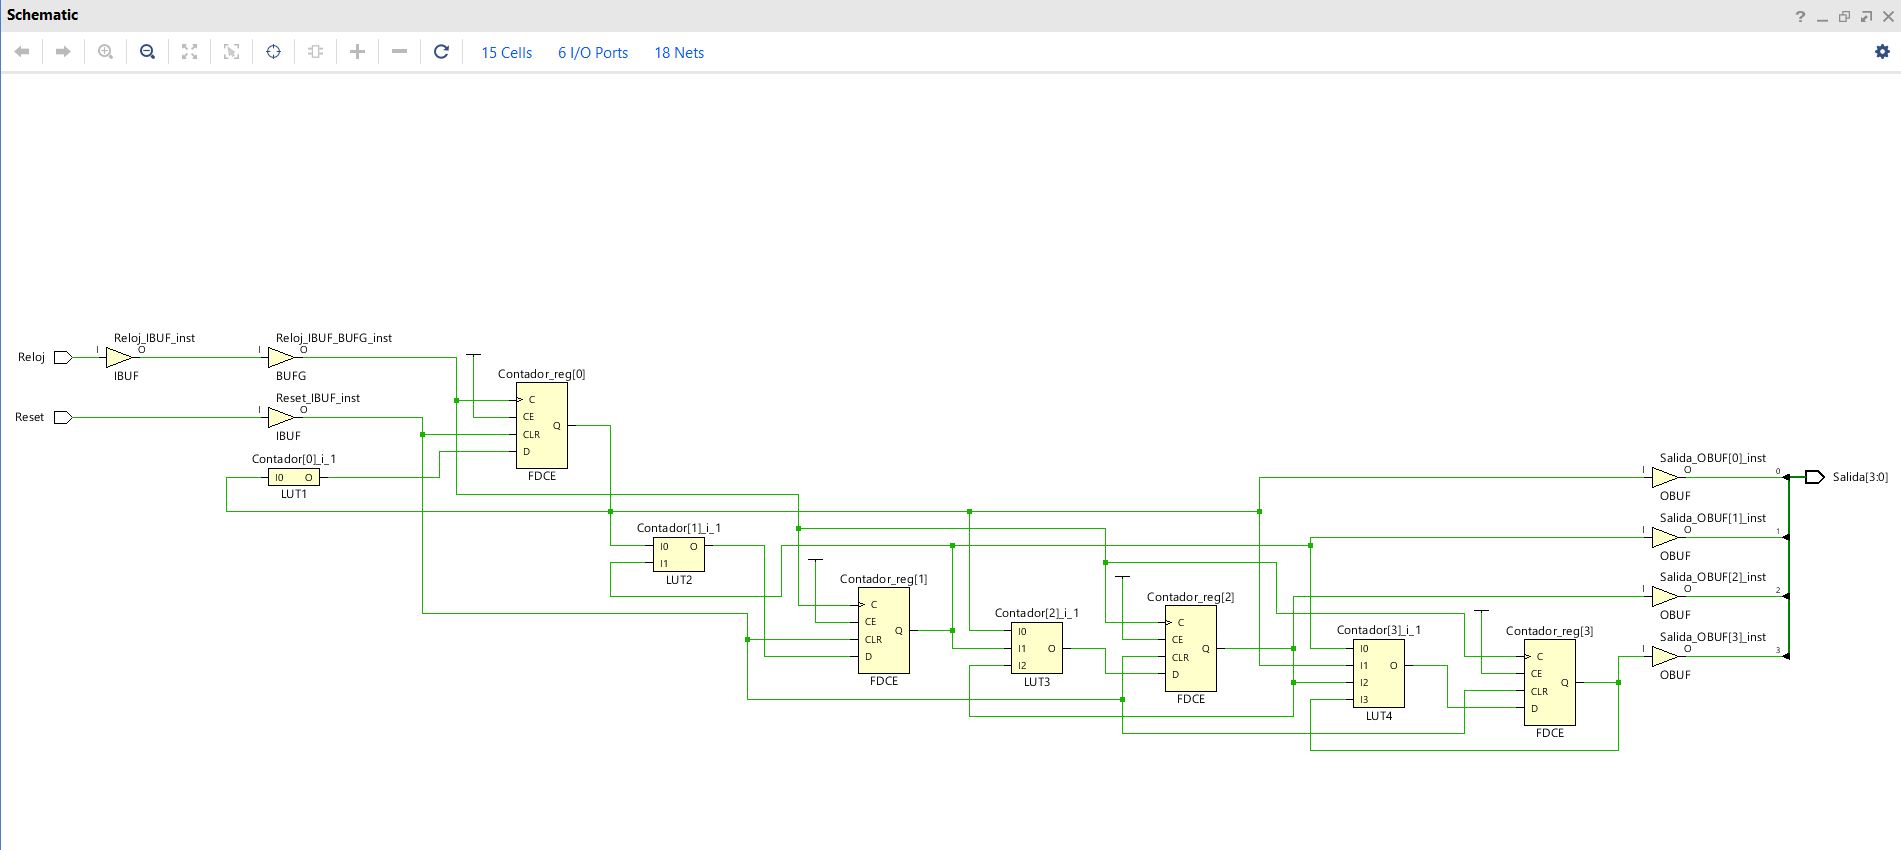
\includegraphics[width = 1\textwidth]{imagenes/netlist1.png}
    \caption{\textit{Netlist Resultante Synthesis}}\label{netlist}
\end{figure}

Para comprobar que el diseño se ejecuta correctamente, realizamos la simulación funcional post-synthesis (Ver Figura \ref{sfps})

\begin{figure}[H]
    \centering
    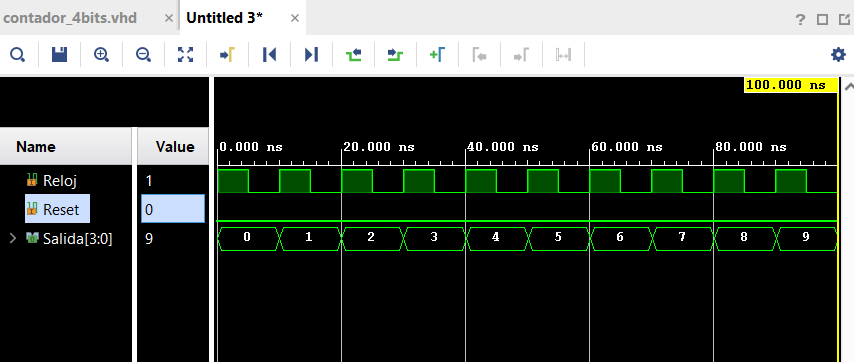
\includegraphics[width = 1\textwidth]{imagenes/simulacionfuncional.png}
    \caption{\textit{Simulación Funcional Post-Synthesis}}\label{sfps}
\end{figure}

Antes de realizar la simulación temporal, deben consultarse los resultados del análisis temporal para determinar la frecuencia máxima de funcionamiento 
y establecer un periodo adecuado para la señal de reloj. Al principio se usó una frecuencia de 125MHz con un reloj de 8ns, pero en el ``Timming Summary'' 
había un apartado de slacks negativos que aunque no daban error, mostraban información de que se podía aumentar la frecuencia máxima a la que trabajaba el 
circuito. Por lo tanto, si bajamos el período del reloj a 3,005ns tendremos una frecuencia de 332.779MHz y como consecuencia ningún slack negativo como se 
muestra en la figura \ref{analisis}.

\begin{figure}[H]
    \centering
    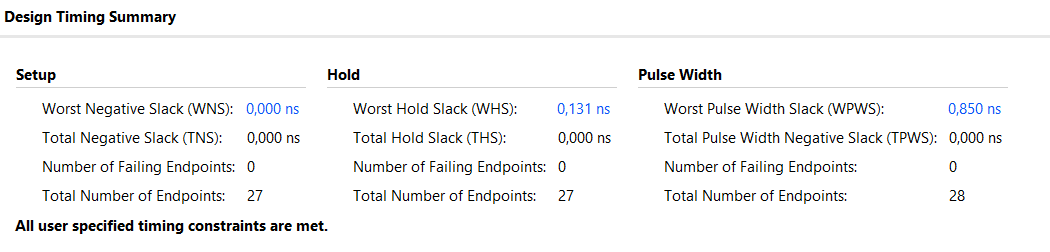
\includegraphics[width = 1\textwidth]{imagenes/analisis.png}
    \caption{\textit{Resumen Temporal Synthesis}}\label{analisis}
\end{figure}

Después de haber ajustado el reloj a la frecuencia máxima a la que puede operar el circuito, comprobamos los retardos que tiene la netlist resultante 
con la simulación temporal post-synthesis (Ver Figura \ref{stps})

\begin{figure}[H]
    \centering
    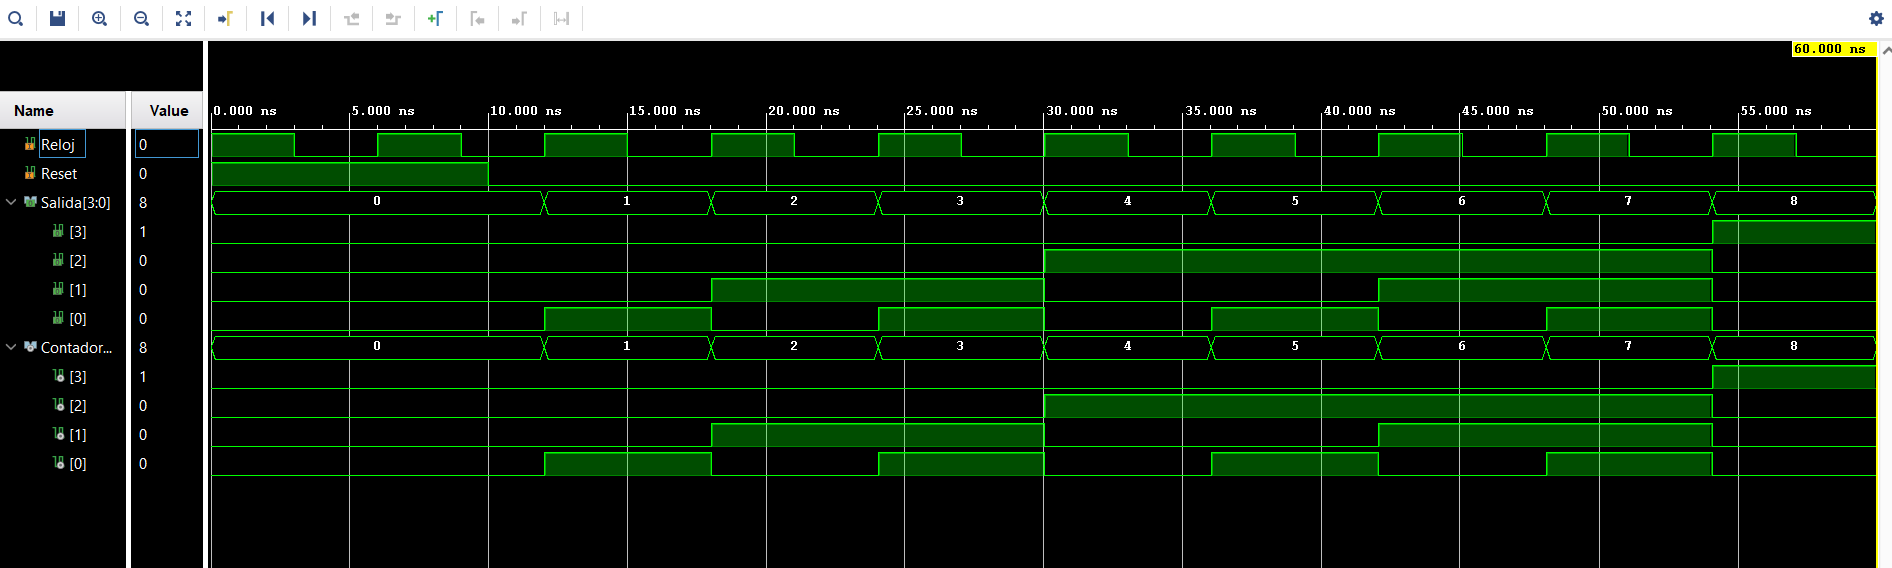
\includegraphics[width = 1\textwidth]{imagenes/simulaciontemporal.png}
    \caption{\textit{Simulación Temporal Post-Synthesis}}\label{stps}
\end{figure}

Ahora pasamos a la fase de implementación (\textit{Implementation}). Para ello, ejecutamos la implementación, y si la plataforma no nos muestra 
ningún error, sólo tenemos que añadir las restricciones de la tarjeta que estamos utilizando (\textit{Add sources} $\rightarrow$ \textit{Add or create constraints}). 
Además hay que asignar los pines correctamente, en este ejemplo, sólo se necesita el reloj, el reset, los botones y los LEDs.

\vspace{1cm}

\begin{lstlisting}
    set_property -dict { PACKAGE_PIN L16   IOSTANDARD LVCMOS33 } [get_ports { clk }]; #IO_L11P_T1_SRCC_35
    create_clock -period 3.005 -name sys_clk_pin -waveform {0.000 1.503} -add [get_ports clk]

    set_property -dict { PACKAGE_PIN G15   IOSTANDARD LVCMOS33 } [get_ports { rst }]; #IO_L19N_T3_VREF_35

    set_property -dict { PACKAGE_PIN R18   IOSTANDARD LVCMOS33 } [get_ports { btn[0] }]; #IO_L20N_T3_34 
    set_property -dict { PACKAGE_PIN P16   IOSTANDARD LVCMOS33 } [get_ports { btn[1] }]; #IO_L24N_T3_34 
    set_property -dict { PACKAGE_PIN V16   IOSTANDARD LVCMOS33 } [get_ports { btn[2] }]; #IO_L18P_T2_34 
    set_property -dict { PACKAGE_PIN Y16   IOSTANDARD LVCMOS33 } [get_ports { btn[3] }]; #IO_L7P_T1_34 

    set_property -dict { PACKAGE_PIN M14   IOSTANDARD LVCMOS33 } [get_ports { led[0] }]; #IO_L23P_T3_35 Sch=LED0
    set_property -dict { PACKAGE_PIN M15   IOSTANDARD LVCMOS33 } [get_ports { led[1] }]; #IO_L23N_T3_35 Sch=LED1
    set_property -dict { PACKAGE_PIN G14   IOSTANDARD LVCMOS33 } [get_ports { led[2] }]; #IO_0_35=Sch=LED2
    set_property -dict { PACKAGE_PIN D18   IOSTANDARD LVCMOS33 } [get_ports { led[3] }]; #IO_L3N_T0_DQS_AD1N_35 Sch=LED3
\end{lstlisting}

Tras realizar esta ejecución, tenemos que volver a comprobar el ``Timming Summary'' para asegurarnos de que no hay slacks negativos (Figura \ref{analisis2}). Viendo 
que los slacks negativos están en positivo, podemos bajar el período del reloj usado para aumentar la frecuencia, quedando el reloj a 2.7ns y la frecuencia a 
370.37MHz.

\begin{figure}[H]
    \centering
    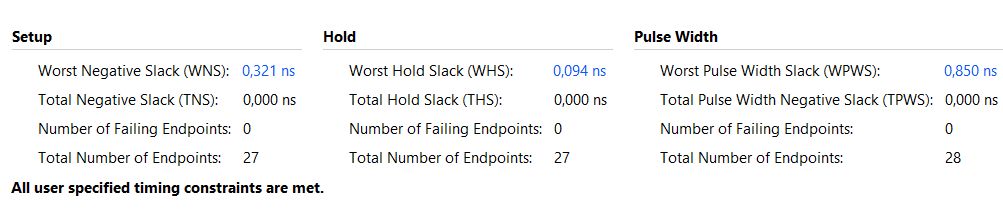
\includegraphics[width = 1\textwidth]{imagenes/analisis2.png}
    \caption{\textit{Resumen Temporal Implementation}}\label{analisis2}
\end{figure}

Y ahora podemos volver a realizar la simulación funcional post-implementation y la temporal post-implementation

\begin{figure}[H]
    \centering
    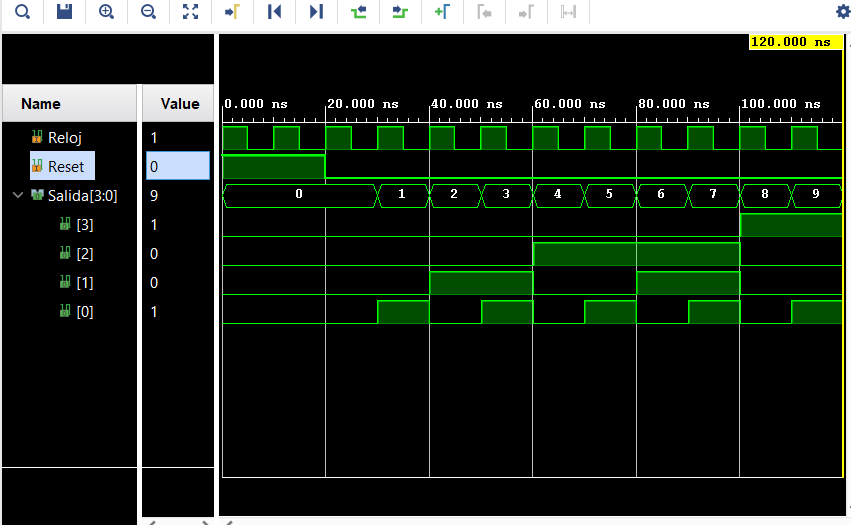
\includegraphics[width = 1\textwidth]{imagenes/simulacionfuncional2.png}
    \caption{\textit{Simulación Funcional Post-Implementation}}\label{sfps1}
\end{figure}

\begin{figure}[H]
    \centering
    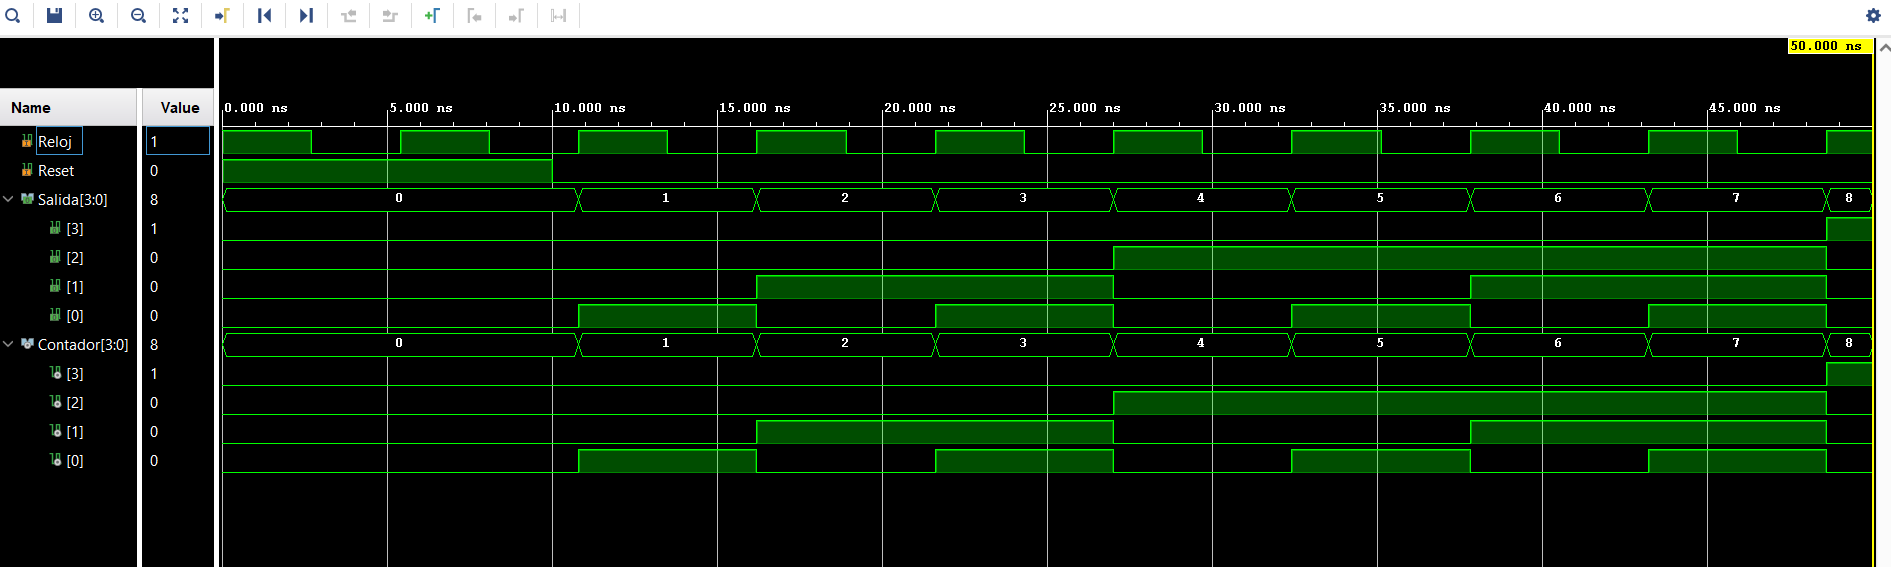
\includegraphics[width = 1\textwidth]{imagenes/simulaciontemporal2.png}
    \caption{\textit{Simulación Temporal Post-Implementation}}\label{stps1}
\end{figure}

Cuando se haya realizado correctamente la ejecución de la implementación, se genera el fichero bitstream y si no hay ningún error se lleva a la FPGA. 
Debido a la frecuencia a la que trabaja la FPGA, la salida de los LEDs no es la del contador, sino una luz verde fija. Para arreglar esto, tenemos 
que añadir un divisor de frecuencias variable cuya frecuencia de salida depende de los valores de 3 entradas.

Pero no basta sólo con añadir este archivo, necesitamos otro archivo que una estos dos anteriores. A continuación se muestra cómo se instancian el 
divisor de frecuencias y el contador de 4 bits.

\begin{lstlisting}
    LIBRARY IEEE;
    USE IEEE.STD_LOGIC_1164.all;
    USE  IEEE.STD_LOGIC_ARITH.all;
    USE  IEEE.STD_LOGIC_UNSIGNED.all;
    
    ENTITY Top IS
        PORT(
            btn      : IN	STD_LOGIC_VECTOR(2 downto 0);
            clk		 : IN	STD_LOGIC;
            rst   	 : IN   STD_LOGIC;
            led      : OUT	STD_LOGIC_VECTOR(0 TO 3));
    END Top;
    
    ARCHITECTURE estructural OF Top IS
    
        COMPONENT Div_Frec is 
        Port(	Velocidad 	: IN 	std_logic_vector(2 downto 0);
                Reloj	    : IN	std_logic;
                Salida		: OUT	std_logic);
        END COMPONENT;
    
        COMPONENT contador_4bits is 
        Port(	Reloj		: IN	std_logic;
                Reset		: IN	std_logic;
                Salida	    : OUT	std_logic_vector(3 downto 0));
        END COMPONENT;
            
        SIGNAL   CKcont : std_logic;
    
    BEGIN
        
    
        DivisorFrecuencia: Div_Frec PORT MAP(
                                    Velocidad => btn,
                                    Reloj =>    clk,
                                    Salida =>   CKcont);
                                    
        Contador4: contador_4bits PORT MAP(
                                    Reloj => CKcont,
                                    Reset => rst,
                                    Salida =>  led);	
    
    END estructural;
\end{lstlisting}

Tras haber añadido estos archivos que completan el diseño del contador, volvemos a realizar los pasos anteriormente dados, 
ejecución de la síntesis, de la implementación y la generación del fichero bitstream. Después lo cargamos en la FPGA y 
ya si se puede ver el contador reflejado en los LEDs de la tarjeta. Además con los interruptores se puede aumentar la frecuencia o 
disminuirla, es decir, la velocidad a la que parpadean los LEDs.
